Distributed PQ monitoring is a common subject in literature\cite{daponte2004transientmeter}\cite{byman2000using}\cite{cristaldi2002distributed}. Projects such as F-NET\cite{zhang2010wide} have demonstrated the utility of Phaser Measurement Unit in monitoring of the US power grid. Distributed PQ recorders such as PQube\cite{von2014micro} have been used in many research applications, from renewable integration, to novel smartgrid designs.

Dense distributed consumer level monitoring, on the order of a meter for $10mi^2$ is not often considered due to cost, privacy, and bandwidth constraints. 

\subsection{OPQBox}

In order to demonstrate our privacy enabled grid visualization method, we developed and deployed five in-house built power quality monitors (OPQBox1). OPQBox1 connects to the user's power outlet, via a step-down transformer and digitizes the resulting signal. While the sampling was controlled by a real-time MCU, waveform analysis was performed by the Raspberry Pi SBC. OPQBox1 computed average frequency and line to neutral voltage at 1 second intervals. By connecting to the resident's 802.11 WIFI, OPQBox1 forwarded both the raw digitized signal as well as the computed frequency and RMS voltage to OPQHub for display. OPQBox1 lacked GPS and used NTP for synchronization. 

\subsection{Deployment}

Five OPQBox1 devices were deployed as a part of an OPQHub pilot study. Two devices were located in residential housing,  two in an apartment building, and one in an office building. As part of the privacy enabled visualization only the office building's location was set in the OPQHub. Devices located in the apartment building were located to the 250mx250m grid square at depth five in the quad tree. Similarly, devices located in houses were constrained to the 500mx500m grid square at the quad tree depth of 4. 

If the frequency or voltage recorder by the OPQBox1 was outside of a set threshold, OPQHub would mark a 1 second measurement as an event if:
\begin{itemize}
\item Frequency deviated by $\pm 0.5Hz$ from the $60Hz$.
\item RMS voltage deviated by $\pm 7V_{rms}$ from the $120V_{rms}$.
\end{itemize}
Voltage events were further classified by severity using the ITIC Curve standard\cite{m:ITIC}. Over 10000 events were recorded, 30 of those events were categorized as an ITIC interruption and 2 were in the prohibited region. However, these events were localized to an individual device. This leads us to believe that the disturbance originated from the consumer's side of the meter. Only 12 events were temporally correlated between multiple devices. An example of such event is shown in Figure \ref{fig:gridwide}. 

\begin{figure}[htbp]
	\centering
	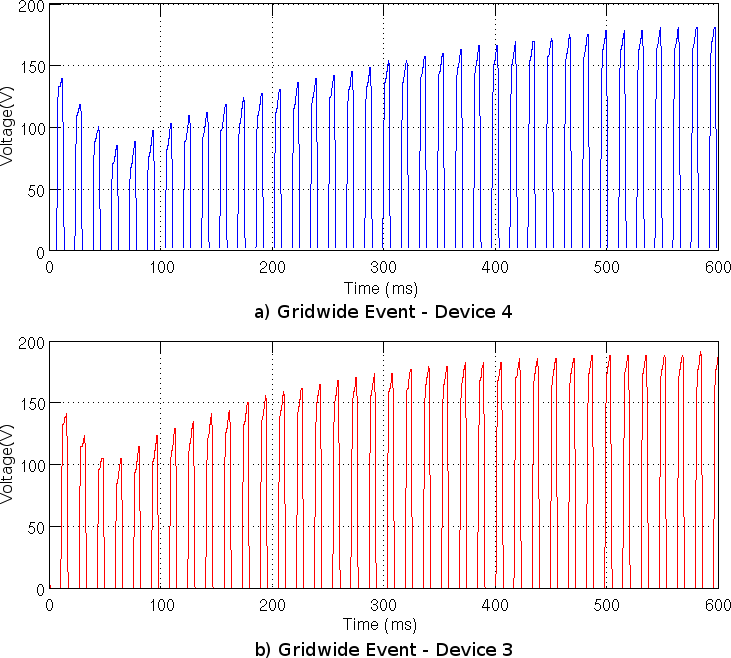
\includegraphics[width=1\columnwidth]{img/gridwide.png}
	\caption{Event recorded by two devices. Only positive voltage is displayed for clarity.}
	\label{fig:gridwide}
\end{figure}

As a part of our pilot study we considered integration of the renewable generation data into OPQHub. Figure \ref{fig:opqbox1} shows the neutral-line voltage trend in green and rooftop solar production in blue. Its worth noting that the the OPQBox1 device which recorded this trend was located in a residential house, 20 miles away from the rooftop solar installation. The first plot in Figure \ref{fig:opqbox1} shows the OPQBox1 recorded voltage in green as well as the solar power production as reported by the Enphase\textregistered {} inverter. During October 15-18 2014, with typical sunny weather, line voltage tracks solar production. During October 18-20, however hurricane Ana passed within 100mi from the island of Oahu. With almost complete cloud cover, rooftop solar production was diminished, and the daily voltage swell was not observed. It is our aim to integrate inverter readings into OPQHub on an opt-in basis.

